% Created by tikzDevice version 0.12 on 2019-04-23 11:27:09
% !TEX encoding = UTF-8 Unicode
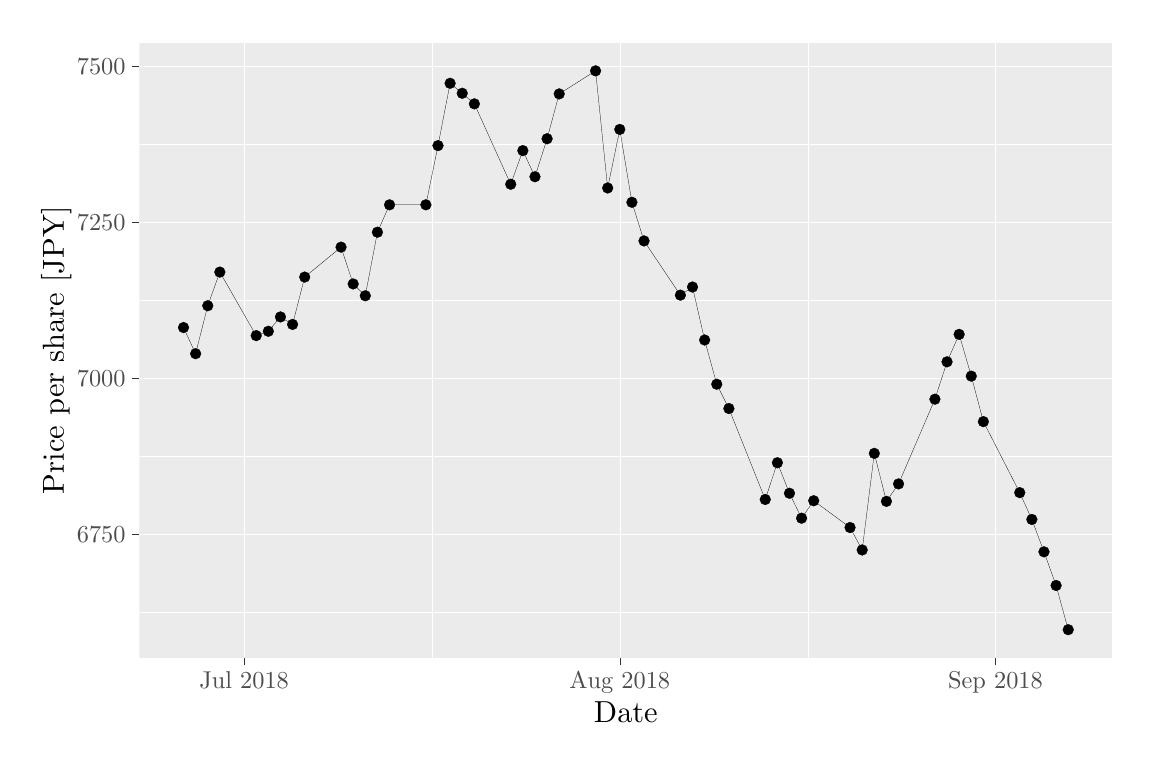
\begin{tikzpicture}[x=1pt,y=1pt]
\definecolor{fillColor}{RGB}{255,255,255}
\path[use as bounding box,fill=fillColor,fill opacity=0.00] (0,0) rectangle (397.48,258.37);
\begin{scope}
\path[clip] (  0.00,  0.00) rectangle (397.48,258.37);
\definecolor{drawColor}{RGB}{255,255,255}
\definecolor{fillColor}{RGB}{255,255,255}

\path[draw=drawColor,line width= 0.1pt,line join=round,line cap=round,fill=fillColor] (  0.00,  0.00) rectangle (397.48,258.37);
\end{scope}
\begin{scope}
\path[clip] ( 40.32, 30.73) rectangle (391.98,252.87);
\definecolor{fillColor}{gray}{0.92}

\path[fill=fillColor] ( 40.32, 30.73) rectangle (391.98,252.87);
\definecolor{drawColor}{RGB}{255,255,255}

\path[draw=drawColor,line width= 0.1pt,line join=round] ( 40.32, 47.35) --
	(391.98, 47.35);

\path[draw=drawColor,line width= 0.1pt,line join=round] ( 40.32,103.64) --
	(391.98,103.64);

\path[draw=drawColor,line width= 0.1pt,line join=round] ( 40.32,159.92) --
	(391.98,159.92);

\path[draw=drawColor,line width= 0.1pt,line join=round] ( 40.32,216.20) --
	(391.98,216.20);

\path[draw=drawColor,line width= 0.1pt,line join=round] (146.08, 30.73) --
	(146.08,252.87);

\path[draw=drawColor,line width= 0.1pt,line join=round] (281.84, 30.73) --
	(281.84,252.87);

\path[draw=drawColor,line width= 0.1pt,line join=round] ( 40.32, 75.50) --
	(391.98, 75.50);

\path[draw=drawColor,line width= 0.1pt,line join=round] ( 40.32,131.78) --
	(391.98,131.78);

\path[draw=drawColor,line width= 0.1pt,line join=round] ( 40.32,188.06) --
	(391.98,188.06);

\path[draw=drawColor,line width= 0.1pt,line join=round] ( 40.32,244.34) --
	(391.98,244.34);

\path[draw=drawColor,line width= 0.1pt,line join=round] ( 78.20, 30.73) --
	( 78.20,252.87);

\path[draw=drawColor,line width= 0.1pt,line join=round] (213.96, 30.73) --
	(213.96,252.87);

\path[draw=drawColor,line width= 0.1pt,line join=round] (349.72, 30.73) --
	(349.72,252.87);
\definecolor{drawColor}{RGB}{0,0,0}

\path[draw=drawColor,line width= 0.1pt,line join=round] ( 56.31,150.01) --
	( 60.69,140.56) --
	( 65.07,157.89) --
	( 69.44,170.05) --
	( 82.58,147.09) --
	( 86.96,148.66) --
	( 91.34,153.84) --
	( 95.72,151.14) --
	(100.10,168.25) --
	(113.24,179.06) --
	(117.62,165.77) --
	(122.00,161.50) --
	(126.38,184.46) --
	(130.76,194.36) --
	(143.89,194.36) --
	(148.27,215.75) --
	(152.65,238.27) --
	(157.03,234.66) --
	(161.41,230.84) --
	(174.55,201.79) --
	(178.93,213.95) --
	(183.31,204.50) --
	(187.69,218.23) --
	(192.07,234.44) --
	(205.21,242.77) --
	(209.58,200.44) --
	(213.96,221.61) --
	(218.34,195.27) --
	(222.72,181.31) --
	(235.86,161.72) --
	(240.24,164.65) --
	(244.62,145.51) --
	(249.00,129.53) --
	(253.38,120.75) --
	(266.52, 87.88) --
	(270.90,101.16) --
	(275.27, 90.13) --
	(279.65, 81.12) --
	(284.03, 87.43) --
	(297.17, 77.75) --
	(301.55, 69.64) --
	(305.93,104.54) --
	(310.31, 87.20) --
	(314.69, 93.51) --
	(327.83,124.12) --
	(332.21,137.63) --
	(336.59,147.54) --
	(340.97,132.45) --
	(345.34,116.02) --
	(358.48, 90.35) --
	(362.86, 80.67) --
	(367.24, 68.97) --
	(371.62, 56.81) --
	(376.00, 40.83);
\definecolor{fillColor}{RGB}{0,0,0}

\path[draw=drawColor,line width= 0.1pt,line join=round,line cap=round,fill=fillColor] ( 56.31,150.01) circle (  1.96);

\path[draw=drawColor,line width= 0.1pt,line join=round,line cap=round,fill=fillColor] ( 60.69,140.56) circle (  1.96);

\path[draw=drawColor,line width= 0.1pt,line join=round,line cap=round,fill=fillColor] ( 65.07,157.89) circle (  1.96);

\path[draw=drawColor,line width= 0.1pt,line join=round,line cap=round,fill=fillColor] ( 69.44,170.05) circle (  1.96);

\path[draw=drawColor,line width= 0.1pt,line join=round,line cap=round,fill=fillColor] ( 82.58,147.09) circle (  1.96);

\path[draw=drawColor,line width= 0.1pt,line join=round,line cap=round,fill=fillColor] ( 86.96,148.66) circle (  1.96);

\path[draw=drawColor,line width= 0.1pt,line join=round,line cap=round,fill=fillColor] ( 91.34,153.84) circle (  1.96);

\path[draw=drawColor,line width= 0.1pt,line join=round,line cap=round,fill=fillColor] ( 95.72,151.14) circle (  1.96);

\path[draw=drawColor,line width= 0.1pt,line join=round,line cap=round,fill=fillColor] (100.10,168.25) circle (  1.96);

\path[draw=drawColor,line width= 0.1pt,line join=round,line cap=round,fill=fillColor] (113.24,179.06) circle (  1.96);

\path[draw=drawColor,line width= 0.1pt,line join=round,line cap=round,fill=fillColor] (117.62,165.77) circle (  1.96);

\path[draw=drawColor,line width= 0.1pt,line join=round,line cap=round,fill=fillColor] (122.00,161.50) circle (  1.96);

\path[draw=drawColor,line width= 0.1pt,line join=round,line cap=round,fill=fillColor] (126.38,184.46) circle (  1.96);

\path[draw=drawColor,line width= 0.1pt,line join=round,line cap=round,fill=fillColor] (130.76,194.36) circle (  1.96);

\path[draw=drawColor,line width= 0.1pt,line join=round,line cap=round,fill=fillColor] (143.89,194.36) circle (  1.96);

\path[draw=drawColor,line width= 0.1pt,line join=round,line cap=round,fill=fillColor] (148.27,215.75) circle (  1.96);

\path[draw=drawColor,line width= 0.1pt,line join=round,line cap=round,fill=fillColor] (152.65,238.27) circle (  1.96);

\path[draw=drawColor,line width= 0.1pt,line join=round,line cap=round,fill=fillColor] (157.03,234.66) circle (  1.96);

\path[draw=drawColor,line width= 0.1pt,line join=round,line cap=round,fill=fillColor] (161.41,230.84) circle (  1.96);

\path[draw=drawColor,line width= 0.1pt,line join=round,line cap=round,fill=fillColor] (174.55,201.79) circle (  1.96);

\path[draw=drawColor,line width= 0.1pt,line join=round,line cap=round,fill=fillColor] (178.93,213.95) circle (  1.96);

\path[draw=drawColor,line width= 0.1pt,line join=round,line cap=round,fill=fillColor] (183.31,204.50) circle (  1.96);

\path[draw=drawColor,line width= 0.1pt,line join=round,line cap=round,fill=fillColor] (187.69,218.23) circle (  1.96);

\path[draw=drawColor,line width= 0.1pt,line join=round,line cap=round,fill=fillColor] (192.07,234.44) circle (  1.96);

\path[draw=drawColor,line width= 0.1pt,line join=round,line cap=round,fill=fillColor] (205.21,242.77) circle (  1.96);

\path[draw=drawColor,line width= 0.1pt,line join=round,line cap=round,fill=fillColor] (209.58,200.44) circle (  1.96);

\path[draw=drawColor,line width= 0.1pt,line join=round,line cap=round,fill=fillColor] (213.96,221.61) circle (  1.96);

\path[draw=drawColor,line width= 0.1pt,line join=round,line cap=round,fill=fillColor] (218.34,195.27) circle (  1.96);

\path[draw=drawColor,line width= 0.1pt,line join=round,line cap=round,fill=fillColor] (222.72,181.31) circle (  1.96);

\path[draw=drawColor,line width= 0.1pt,line join=round,line cap=round,fill=fillColor] (235.86,161.72) circle (  1.96);

\path[draw=drawColor,line width= 0.1pt,line join=round,line cap=round,fill=fillColor] (240.24,164.65) circle (  1.96);

\path[draw=drawColor,line width= 0.1pt,line join=round,line cap=round,fill=fillColor] (244.62,145.51) circle (  1.96);

\path[draw=drawColor,line width= 0.1pt,line join=round,line cap=round,fill=fillColor] (249.00,129.53) circle (  1.96);

\path[draw=drawColor,line width= 0.1pt,line join=round,line cap=round,fill=fillColor] (253.38,120.75) circle (  1.96);

\path[draw=drawColor,line width= 0.1pt,line join=round,line cap=round,fill=fillColor] (266.52, 87.88) circle (  1.96);

\path[draw=drawColor,line width= 0.1pt,line join=round,line cap=round,fill=fillColor] (270.90,101.16) circle (  1.96);

\path[draw=drawColor,line width= 0.1pt,line join=round,line cap=round,fill=fillColor] (275.27, 90.13) circle (  1.96);

\path[draw=drawColor,line width= 0.1pt,line join=round,line cap=round,fill=fillColor] (279.65, 81.12) circle (  1.96);

\path[draw=drawColor,line width= 0.1pt,line join=round,line cap=round,fill=fillColor] (284.03, 87.43) circle (  1.96);

\path[draw=drawColor,line width= 0.1pt,line join=round,line cap=round,fill=fillColor] (297.17, 77.75) circle (  1.96);

\path[draw=drawColor,line width= 0.1pt,line join=round,line cap=round,fill=fillColor] (301.55, 69.64) circle (  1.96);

\path[draw=drawColor,line width= 0.1pt,line join=round,line cap=round,fill=fillColor] (305.93,104.54) circle (  1.96);

\path[draw=drawColor,line width= 0.1pt,line join=round,line cap=round,fill=fillColor] (310.31, 87.20) circle (  1.96);

\path[draw=drawColor,line width= 0.1pt,line join=round,line cap=round,fill=fillColor] (314.69, 93.51) circle (  1.96);

\path[draw=drawColor,line width= 0.1pt,line join=round,line cap=round,fill=fillColor] (327.83,124.12) circle (  1.96);

\path[draw=drawColor,line width= 0.1pt,line join=round,line cap=round,fill=fillColor] (332.21,137.63) circle (  1.96);

\path[draw=drawColor,line width= 0.1pt,line join=round,line cap=round,fill=fillColor] (336.59,147.54) circle (  1.96);

\path[draw=drawColor,line width= 0.1pt,line join=round,line cap=round,fill=fillColor] (340.97,132.45) circle (  1.96);

\path[draw=drawColor,line width= 0.1pt,line join=round,line cap=round,fill=fillColor] (345.34,116.02) circle (  1.96);

\path[draw=drawColor,line width= 0.1pt,line join=round,line cap=round,fill=fillColor] (358.48, 90.35) circle (  1.96);

\path[draw=drawColor,line width= 0.1pt,line join=round,line cap=round,fill=fillColor] (362.86, 80.67) circle (  1.96);

\path[draw=drawColor,line width= 0.1pt,line join=round,line cap=round,fill=fillColor] (367.24, 68.97) circle (  1.96);

\path[draw=drawColor,line width= 0.1pt,line join=round,line cap=round,fill=fillColor] (371.62, 56.81) circle (  1.96);

\path[draw=drawColor,line width= 0.1pt,line join=round,line cap=round,fill=fillColor] (376.00, 40.83) circle (  1.96);
\end{scope}
\begin{scope}
\path[clip] (  0.00,  0.00) rectangle (397.48,258.37);
\definecolor{drawColor}{gray}{0.30}

\node[text=drawColor,anchor=base east,inner sep=0pt, outer sep=0pt, scale=  0.88] at ( 35.37, 72.46) {6750};

\node[text=drawColor,anchor=base east,inner sep=0pt, outer sep=0pt, scale=  0.88] at ( 35.37,128.75) {7000};

\node[text=drawColor,anchor=base east,inner sep=0pt, outer sep=0pt, scale=  0.88] at ( 35.37,185.03) {7250};

\node[text=drawColor,anchor=base east,inner sep=0pt, outer sep=0pt, scale=  0.88] at ( 35.37,241.31) {7500};
\end{scope}
\begin{scope}
\path[clip] (  0.00,  0.00) rectangle (397.48,258.37);
\definecolor{drawColor}{gray}{0.20}

\path[draw=drawColor,line width= 0.1pt,line join=round] ( 37.57, 75.50) --
	( 40.32, 75.50);

\path[draw=drawColor,line width= 0.1pt,line join=round] ( 37.57,131.78) --
	( 40.32,131.78);

\path[draw=drawColor,line width= 0.1pt,line join=round] ( 37.57,188.06) --
	( 40.32,188.06);

\path[draw=drawColor,line width= 0.1pt,line join=round] ( 37.57,244.34) --
	( 40.32,244.34);
\end{scope}
\begin{scope}
\path[clip] (  0.00,  0.00) rectangle (397.48,258.37);
\definecolor{drawColor}{gray}{0.20}

\path[draw=drawColor,line width= 0.1pt,line join=round] ( 78.20, 27.98) --
	( 78.20, 30.73);

\path[draw=drawColor,line width= 0.1pt,line join=round] (213.96, 27.98) --
	(213.96, 30.73);

\path[draw=drawColor,line width= 0.1pt,line join=round] (349.72, 27.98) --
	(349.72, 30.73);
\end{scope}
\begin{scope}
\path[clip] (  0.00,  0.00) rectangle (397.48,258.37);
\definecolor{drawColor}{gray}{0.30}

\node[text=drawColor,anchor=base,inner sep=0pt, outer sep=0pt, scale=  0.88] at ( 78.20, 19.72) {Jul 2018};

\node[text=drawColor,anchor=base,inner sep=0pt, outer sep=0pt, scale=  0.88] at (213.96, 19.72) {Aug 2018};

\node[text=drawColor,anchor=base,inner sep=0pt, outer sep=0pt, scale=  0.88] at (349.72, 19.72) {Sep 2018};
\end{scope}
\begin{scope}
\path[clip] (  0.00,  0.00) rectangle (397.48,258.37);
\definecolor{drawColor}{RGB}{0,0,0}

\node[text=drawColor,anchor=base,inner sep=0pt, outer sep=0pt, scale=  1.10] at (216.15,  7.44) {Date};
\end{scope}
\begin{scope}
\path[clip] (  0.00,  0.00) rectangle (397.48,258.37);
\definecolor{drawColor}{RGB}{0,0,0}

\node[text=drawColor,rotate= 90.00,anchor=base,inner sep=0pt, outer sep=0pt, scale=  1.10] at ( 13.08,141.80) {Price per share [JPY]};
\end{scope}
\end{tikzpicture}
